% Discussion, v3. Restructured around the estimation thesis: 5.1 the design rule
% (division of labour), 5.2 the estimation demonstration and its limits (new),
% 5.3 decodability versus estimability, 5.4 limitations and outlook. Voice per
% the Fukami calibration; every quoted number a macros_v3 macro; the v2.1
% spatial-tier quantitative material and the wake-code figure leave this section
% (the v3 numbers live in Section 4.6; the decode galleries go to Appendix C).
% D244: honest T2b framing, no overselling, Y mentioned only. D243: the merit
% tie is reported as seed-fragile; readability tie robust.
% Session 39 (comparison-led reframe, paper_redesign.md section 5): capacity
% caveat (reviewer risk R3) added to 5.1; the "Choosing the estimator" ladder
% subsection is demotion-bound to the appendix per D-B (flagged inline).

\subsection{What a wall-estimable state must contain}
\label{sec:disc_mechanism}
\label{sec:disc_caveat}

The comparison has a direction, and the deployment ladder of
figure~\ref{fig:deployment_ladder} reads it off. On the decoded field the three
families are indistinguishable, the energy-optimal linear basis as sharp as the
nonlinear states, so field fidelity does not separate them. The separation opens
at the first task that needs the wake, the observable read-out, where the linear
basis loses the load at the impact instant and neither it nor the reconstruction
reads the wake; and it widens at every step toward deployment. Through the impact
the reconstruction's forecast collapses and the linear basis fades; recovering
the state from sparse wall pressure, the predictive latent carries the most
physics from a less recoverable state; and under assimilation at the strong-gust
boundary the predictive filter is the only one that does not diverge on nearly
every encounter. The predictive state is the single family that holds all the way
down the chain, and that is the design rule stated operationally: a state earns
its place at deployment not by rendering the field but by remaining readable,
forecastable, wall-recoverable and assimilable at once.

\begin{figure}
  \centering
  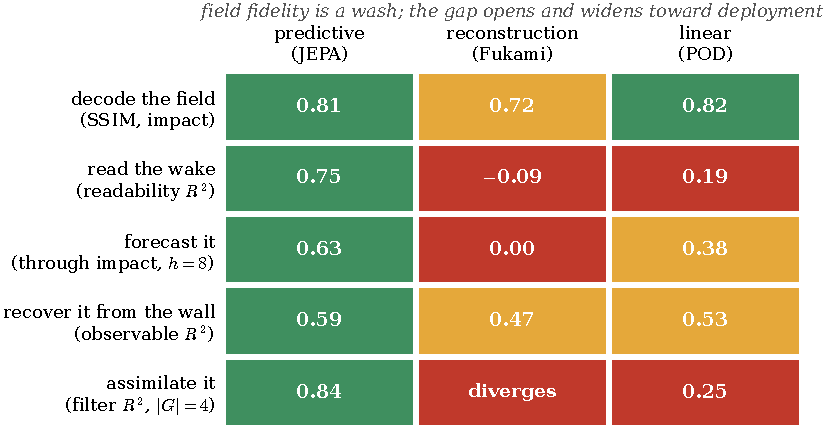
\includegraphics[width=0.92\linewidth]{sections/figures/results/fig_deployment_ladder.pdf}
  \caption{The deployment ladder. Each rung is a task a wall-borne reduced state
  must perform, ordered top to bottom by increasing deployment demand, and each
  cell is the representative metric from the section that establishes it: field
  SSIM at impact (\S\ref{sec:res_compress}), wake readability
  (\S\ref{sec:res_carries}), through-impact forecast merit at $h = 8$
  (\S\ref{sec:res_forecast}), wall observable recovery (\S\ref{sec:res_wallobs})
  and filter closure at the $|G| = 4$ boundary (\S\ref{sec:res_estimation});
  colour marks whether the family holds the rung. Field fidelity does not
  separate the families; the predictive state is the only one that holds every
  rung to deployment. The reconstruction column is the Fukami lineage, its field
  cell the wake-headed variant that alone carries a decoder; at $|G| = 4$ it
  diverges on almost every encounter.}
  \label{fig:deployment_ladder}
\end{figure}

The central result is a design rule for a reduced state that a wall-pressure
estimator can track. Such a state must carry the wake observables that govern the
post-impact transient, must be organised so that a forward model can advance it
without leaving its own support, and must be recoverable from the surface pressure
that is the only measurement a vehicle carries. These three requirements are
supplied by different ingredients, and separating them is the paper's
contribution. Observable supervision on the wake supplies the first, the
instantaneous readability, and, less obviously, much of the second: it
concentrates the encoded variance into a low-rank subspace aligned with the
observables, and the forward rollout, trained and living in that subspace, stays
in distribution, where an anti-collapse regulariser applied to a bare
reconstruction produces a near-isotropic latent with no protected subspace and a
rollout that leaks into the directions the training data never constrained
(\S\ref{sec:res_rollout}). The mechanism is geometric, and it refines our earlier
reading, which credited the anti-collapse term: a reconstruction objective fixes
the latent only up to a diffeomorphism \citep{kelshaw2024}, the anti-collapse term
on its own drives the latent toward isotropy \citep{broustail2026}, and it is the
supervision that pins the variance onto the observable-aligned directions the
rollout respects. The multi-step predictive objective supplies the rest of the
second requirement, the long-horizon stability that a single-step objective and an
objective-free supervised encoder both lack, and, across retrains, the reliability
of the forecast itself (\S\ref{sec:disc_limits}). The third requirement, wall
recoverability, is where energy and information part company: the reconstruction
latent is the most recoverable in raw variance but the least in physics, while the
predictive latent carries the most wall-recoverable physics
(\S\ref{sec:res_wall}), so the coefficient state a controller would want is not
the one a reconstruction objective produces.

The wake, and not the forces, is where these requirements separate the families,
and the coordinate-level reading of \S\ref{sec:res_code} explains why.
The forces are carried redundantly in every family, so an energy or reconstruction
objective retains the force signature of an encounter without retaining the
distributed combination of coordinates that carries the vorticity redistribution
producing it. The gust parameters alone predict the forces well and fail on the
wake at the readout horizon, so a state can look accurate on the load while
carrying none of the physics the load is built from, which is exactly the failure
mode the estimation results expose. The linear basis, for its part, remains
genuinely useful: it is competitive on the body forces, amplitude-accurate in
reconstruction, and it holds the shedding clock as well as the predictive latent
(\S\ref{sec:res_latent_physics}); the result is not that POD is obsolete but that
no linear projection reaches the wake at any dimension we tested.

One caveat is inherited from the compactness-versus-forecast comparison that
motivates this study \citep{solerarico_compactness_underreview}: a more
expressive predictor might narrow the forecast gaps between the families. Three
controls argue that the ordering is a property of the representations rather than
of an underpowered predictor. The shared forecaster was capacity-selected on the
\ValSplit{} set, a sequence-LSTM variant included; the matched autoregressive
transformer diverges on the published-recipe latents at equal recipe and budget,
so its failure is not a capacity artefact; and a per-family tuned recovery
estimator raises every family without changing their order (supplementary
material). The orderings reported here are therefore floors set by the
representation, not ceilings set by the predictor.

\subsection{The estimation demonstration and its limits}
\label{sec:disc_estimation}

The filter turns the design rule into a working estimator: from eight
wall-pressure taps and no field measurement it tracks the load through the
encounter and extends the usable gust-intensity range beyond every static
inverse, realising the online-estimation pathway the extreme-aerodynamic control
literature has named \citep{fukami2024control,mousavi2025,eldredge2025guide}. We
are deliberate about its limits, and the first is one the family comparison
forces: the in-range load-tracking is a property of sequential estimation on a
nonlinear latent generally, not of this state, so the paper does not rest the
representational claim on it. What the predictive state contributes to the
estimator is the strong-gust boundary, the calibration margin, and a tracked
state whose coordinates carry the wake; what no state yet contributes is a
filtered wake estimate, since the analysis wake closure is below the mean
predictor for every family. Its recoverability advantage over a raw
high-dimensional field latent is real but modest (\S\ref{sec:res_wall}), so the
case for the coefficient state rests on the physics-recovery ordering and the
envelope, not on a large recoverability margin. Its point tracking is good but its uncertainty is under-dispersed at the
strongest and widest gusts, where the innovations are temporally correlated and
the ensemble collapses. The visibility analysis suggests the mechanism: the
forward model has large gain along the data-unconstrained near-null directions it
never learned to damp, and those inject spread-consuming noise during
assimilation. This points to a calibrated process and observation noise model,
rather than covariance inflation, as the outstanding requirement, and we report
the filter as a feasibility demonstration with a characterised soft spot, not as a
deployed estimator.

The delay-embedding view names the deployment knob and its limit. Because the
encounter is low-dimensional, the state can be tracked from few taps read over a
short window, which is the sensing budget a small vehicle could carry; the trade
between tap count and window length is explicit for the static reconstruction
(\S\ref{sec:res_delays}), so a sensor-poor platform can in principle compensate
with a longer window within the encounter's own timescale. The frozen filter does
not inherit that trade, because its innovation rank, not the embedding, is what
binds at reduced tap count, and the two statements together sharpen the same
conclusion: the noise model, not the sensor count, is the binding constraint. The
limit that no budget escapes is the growth of the encounter's effective dimension
with gust strength. Read through delay coordinates the encounter is an
intermittently forced low-dimensional system \citep{brunton2017chaos}, the
baseline shedding carrying the delay-coordinate dynamics and the vortex impact
acting as a forcing whose amplitude is the gust ratio, which is consistent with
the envelope being organised by $|G|$: no fixed sensing budget embeds the
strongest, most three-dimensional encounters, which is why the envelope closes
where it does (\S\ref{sec:res_envelope}).

\subsection{Decodability versus estimability}
\label{sec:disc_decode}

A reduced state can be optimised for two deployments that pull apart. A spatially
resolved latent decodes the vorticity field more sharply than the coefficient
state, but it is of far higher dimension than the wall measurement and so is not
recoverable from a sparse set of pressure taps. The coefficient state decodes the
field less sharply and is the object a wall-pressure filter can track. We therefore
separate the two roles: the coefficient state is the estimable, forward-usable
object this paper is about, and the field-resolved latent is a decodability
instrument rather than an estimation target. Pooling the encoder onto the
coefficient state costs field fidelity across every family, by
$\PfourSsimDeltaJepa$ in decode similarity and $\PfourMeritDeltaJepa$ in
fitted-operator forecast merit for the predictive latent (supplementary material),
and it gains nothing in wall recoverability that the coefficient state does not
already have. The state a controller would carry is therefore not the one a
field-reconstruction objective produces.

\subsection{Limitations and outlook}
\label{sec:disc_limits}
\label{sec:disc_control}
\label{sec:disc_outlook}

Five limitations bound the claims. First, the attribution of the instantaneous
results is unglamorous: the wake readability is supplied by the
observable supervision and its tie between the predictive and reconstructive
wake-headed states is seed-robust ($\SeedWakeJepaVec \pm \SeedWakeSdJepaVec$
against $\SeedWakeAeWake \pm \SeedWakeSdAeWake$).
% REVIEW-CLAIM: (Session 36, Track M1, D310) the suited-operator "narrow lead"
% this passage previously cautioned against is gone from the main text; the
% shared-operator recomputation makes the tie explicit, and the earlier U-Net
% seed study now corroborates rather than qualifies it.
The shared-operator forecast merit of \S\ref{sec:res_closure} shows the same
picture dynamically: over three operator seeds the three wake-headed states are
statistically indistinguishable, with overlapping case-clustered intervals. An
earlier seed study of the fitted merit, run under the residual U-Net operator
as a stability check, cautions the same way: the supervised
control is seed-fragile (spread $\SeedMeritSdSupOnly$, with one healthy retrain in
three collapsing), the predictive latent is tighter but not the sharpest
($\pm \SeedMeritSdJepaVec$), and the family means overlap. No fitted-operator
margin between the wake-headed states
is therefore decisive on its own. The defensible dynamical claim rests instead
on the co-trained model and its rollout: the \PredState's own predictor forecasts
better than the shared operator extracts from any latent at short horizon
(\S\ref{sec:res_closure}), and the
multi-step objective confers long-horizon stability and lower drift, not a larger
instantaneous readability margin. Second, the wall-normal offset $Y$ remains the least
resolved release parameter because the training mass concentrates near
$Y \approx 0$; the additional cases make it weakly readable where it was
unreadable before (\S\ref{sec:res_latent_physics}), and we note this without
leaning on it. Third, the $|G| = 4$ extrapolation degrades for a physical reason:
the encoder observes a single mid-plane vorticity slice whose information no
longer determines the three-dimensional dynamics there
(\S\ref{sec:flow_physics}), so the \BoundarySplit{} set marks the observability boundary of that
representation, not a parametric-generalisation claim, and the filter meets the
same boundary from the sensing side (\S\ref{sec:res_envelope}). Fourth, the
visualisation decoder is a diagnostic on the frozen encoder, never part of the
predictive loss, and the pooled coefficient state trades decode sharpness for
estimability by construction (\S\ref{sec:disc_decode}). Fifth, and foremost for
what comes next, the filter's calibration is the priority open problem: its
uncertainty is under-dispersed at the strongest gusts, and the natural next step
is a learned or physically motivated process and observation covariance, ahead of
any closed-loop use.

These limitations come into sharpest focus against the use the architecture is
meant for. The predictor is, by construction, a latent dynamics function of the
kind an estimator or controller requires, the latent is orders of magnitude
cheaper to advance than the field, and the filter demonstrates the estimation half
of that loop from the wall alone. Closed-loop actuation is outside the present
evidence: the predictor is trained to forecast observed encounters within the
training envelope, and predicting how an encounter would differ under intervention
is a task its training does not address. The contribution is narrow by design, a
controlled comparison and a frozen-filter characterisation on a single parametric
flow, and what it establishes is bounded accordingly: a wall-estimable,
forward-usable coefficient state, the ingredients that produce it, and the
gust-intensity envelope over which a fixed sensing budget can follow it. The
natural next steps are the noise model above and the same matched-estimator
protocol on other parametric flows, to test how general the estimability ordering
reported here actually is.
